% ==========================================
% Delta Lake Introduction - Google Theme
% Day 4 - Databricks 14-Days AI Challenge
% ==========================================

\documentclass[aspectratio=169,11pt]{beamer}

% ==========================================
% PACKAGES
% ==========================================
\usepackage[utf8]{inputenc}
\usepackage[T1]{fontenc}
\usepackage{lmodern}
\usepackage{graphicx}
\usepackage{booktabs}
\usepackage{tikz}
\usepackage{fontawesome5}
\usepackage{listings}
\usepackage{hyperref}
\usepackage{array}
\usepackage{colortbl}
\usepackage{tcolorbox}
\usepackage{xcolor}
\usepackage{tabularx}
\usepackage{adjustbox}

% ==========================================
% GOOGLE COLOR PALETTE
% ==========================================
\definecolor{GoogleBlue}{RGB}{66, 133, 244}
\definecolor{GoogleRed}{RGB}{234, 67, 53}
\definecolor{GoogleYellow}{RGB}{251, 188, 5}
\definecolor{GoogleGreen}{RGB}{52, 168, 83}
\definecolor{GoogleGray}{RGB}{95, 99, 104}
\definecolor{GoogleLightGray}{RGB}{241, 243, 244}
\definecolor{GoogleDarkGray}{RGB}{32, 33, 36}
\definecolor{GoogleWhite}{RGB}{255, 255, 255}

% ==========================================
% BEAMER THEME CONFIGURATION
% ==========================================
\usetheme{default}
\usecolortheme{default}
\usefonttheme{professionalfonts}

% Remove navigation symbols
\setbeamertemplate{navigation symbols}{}

% Set colors
\setbeamercolor{structure}{fg=GoogleBlue}
\setbeamercolor{title}{fg=GoogleWhite}
\setbeamercolor{subtitle}{fg=GoogleWhite}
\setbeamercolor{author}{fg=GoogleWhite}
\setbeamercolor{date}{fg=GoogleWhite}
\setbeamercolor{institute}{fg=GoogleWhite}
\setbeamercolor{frametitle}{fg=GoogleDarkGray,bg=GoogleWhite}
\setbeamercolor{background canvas}{bg=GoogleWhite}
\setbeamercolor{normal text}{fg=GoogleDarkGray}
\setbeamercolor{itemize item}{fg=GoogleBlue}
\setbeamercolor{itemize subitem}{fg=GoogleRed}
\setbeamercolor{itemize subsubitem}{fg=GoogleGreen}
\setbeamercolor{block title}{fg=GoogleWhite,bg=GoogleBlue}
\setbeamercolor{block body}{fg=GoogleDarkGray,bg=GoogleLightGray}
\setbeamercolor{alerted text}{fg=GoogleRed}

% Bullet styles
\setbeamertemplate{itemize item}{\textcolor{GoogleBlue}{\textbullet}}
\setbeamertemplate{itemize subitem}{\textcolor{GoogleRed}{\textbullet}}
\setbeamertemplate{itemize subsubitem}{\textcolor{GoogleGreen}{\textbullet}}

% ==========================================
% HEADER WITH SLIDE NUMBER AND TITLE
% ==========================================
\setbeamertemplate{frametitle}{%
    \vspace{0.3cm}
    \begin{beamercolorbox}[wd=\paperwidth,ht=1cm,dp=0.3cm]{frametitle}
        \hspace{0.5cm}
        
\begin{tikzpicture}[remember picture, overlay]
            \fill[GoogleBlue] (0,0) circle (0.25cm);
            \node[text=white,font=\small\bfseries] at (0,0) {\insertframenumber};
        \end{tikzpicture}
        \hspace{0.5cm}
        {\Large\bfseries\insertframetitle}
    \end{beamercolorbox}
    \begin{tikzpicture}[remember picture,overlay]
        \draw[GoogleBlue, line width=2pt] (0.3,-0.1) -- (\paperwidth-0.3,-0.1);
    \end{tikzpicture}
}

% ==========================================
% FOOTER CONFIGURATION
% ==========================================
\setbeamertemplate{footline}{%
    \leavevmode%
    \hbox{%
        % Left: Easy AI Labs
        \begin{beamercolorbox}[wd=.33\paperwidth,ht=2.5ex,dp=1ex,left]{author in head/foot}%
            \hspace{0.5cm}
            \textcolor{GoogleBlue}{\faIcon{robot}}
            \textcolor{GoogleGray}{\href{https://easy-ai-labs.lovable.app/}{\small Easy AI Labs}}
        \end{beamercolorbox}%
        % Center: Yash Kavaiya
        \begin{beamercolorbox}[wd=.34\paperwidth,ht=2.5ex,dp=1ex,center]{title in head/foot}%
            \textcolor{GoogleRed}{\faIcon{user}}
            \textcolor{GoogleGray}{\href{https://www.linkedin.com/in/yashkavaiya}{\small Yash Kavaiya}}
        \end{beamercolorbox}%
        % Right: Gen AI Guru
        \begin{beamercolorbox}[wd=.33\paperwidth,ht=2.5ex,dp=1ex,right]{date in head/foot}%
            \textcolor{GoogleGreen}{\faIcon{graduation-cap}}
            \textcolor{GoogleGray}{\href{https://www.linkedin.com/company/genai-guru}{\small Gen AI Guru}}
            \hspace{0.5cm}
        \end{beamercolorbox}%
    }%
    \vskip0pt%
}

% ==========================================
% CODE LISTING STYLE
% ==========================================
\lstset{
    basicstyle=\ttfamily\scriptsize,
    keywordstyle=\color{GoogleBlue}\bfseries,
    stringstyle=\color{GoogleGreen},
    commentstyle=\color{GoogleGray}\itshape,
    backgroundcolor=\color{GoogleLightGray},
    frame=single,
    framerule=0pt,
    breaklines=true,
    showstringspaces=false,
    tabsize=2,
    numbers=none,
    xleftmargin=0.3cm,
    xrightmargin=0.3cm,
    aboveskip=0.3cm,
    belowskip=0.2cm
}

% ==========================================
% CUSTOM BOX STYLES
% ==========================================
\tcbset{
    googlebox/.style={
        colback=GoogleLightGray,
        colframe=GoogleBlue,
        fonttitle=\bfseries,
        boxrule=1pt,
        arc=3pt,
        left=5pt,
        right=5pt,
        top=5pt,
        bottom=5pt
    }
}

% ==========================================
% TITLE PAGE TEMPLATE
% ==========================================
\setbeamertemplate{title page}{
    
\begin{tikzpicture}[remember picture,overlay]
        \fill[GoogleBlue] (current page.north west) rectangle (current page.south east);
        % Decorative circles
        \fill[GoogleRed,opacity=0.3] (12,-6) circle (3cm);
        \fill[GoogleYellow,opacity=0.3] (-2,1) circle (2cm);
        \fill[GoogleGreen,opacity=0.3] (14,2) circle (2.5cm);
    \end{tikzpicture}
    \vspace{1.5cm}
    \begin{center}
        \textcolor{GoogleWhite}{\Huge\bfseries\inserttitle}\\[0.5cm]
        \textcolor{GoogleYellow}{\Large\insertsubtitle}\\[1cm]
        \textcolor{GoogleWhite}{\large\insertauthor}\\[0.3cm]
        \textcolor{GoogleLightGray}{\small\insertinstitute}\\[0.5cm]
        \textcolor{GoogleLightGray}{\small\insertdate}
    \end{center}
}

% ==========================================
% DOCUMENT INFORMATION
% ==========================================
\title{Delta Lake Introduction}
\subtitle{Comprehensive Guide to Data Lake Reliability}
\author{Databricks 14-Days AI Challenge}
\institute{Day 4 - Building the Lakehouse Foundation}
\date{\today}

% ==========================================
% DOCUMENT BEGIN
% ==========================================
\begin{document}

% ==========================================
% TITLE SLIDE
% ==========================================
{
\setbeamertemplate{footline}{}
\begin{frame}[plain]
    \titlepage
\end{frame}
}

% ==========================================
% TABLE OF CONTENTS
% ==========================================
\begin{frame}{Agenda}
    \begin{columns}[T]
        \begin{column}{0.48\textwidth}
            \textcolor{GoogleBlue}{\faIcon{layer-group}} \textbf{Core Concepts}
            \begin{itemize}
                \item What is Delta Lake?
                \item ACID Transactions
                \item Schema Enforcement
            \end{itemize}
            \vspace{0.5cm}
            \textcolor{GoogleRed}{\faIcon{exchange-alt}} \textbf{Comparisons}
            \begin{itemize}
                \item Delta vs Parquet
            \end{itemize}
        \end{column}
        \begin{column}{0.48\textwidth}
            \textcolor{GoogleGreen}{\faIcon{code}} \textbf{Practical Tasks}
            \begin{itemize}
                \item Convert CSV to Delta
                \item Create Delta Tables
                \item Test Schema Enforcement
                \item Handle Duplicate Inserts
            \end{itemize}
            \vspace{0.5cm}
            \textcolor{GoogleYellow}{\faIcon{book}} \textbf{Reference}
            \begin{itemize}
                \item Quick Reference Guide
            \end{itemize}
        \end{column}
    \end{columns}
\end{frame}

% ==========================================
% SECTION 1: WHAT IS DELTA LAKE?
% ==========================================
\begin{frame}{What is Delta Lake?}
    \begin{tcolorbox}[googlebox, title={\textcolor{white}{Definition}}]
        Delta Lake is an \textbf{open-source storage layer} that brings reliability, performance, and governance to data lakes. It runs on top of your existing data lake infrastructure and is fully compatible with Apache Spark APIs.
    \end{tcolorbox}
    
    \vspace{0.5cm}
    
    \begin{columns}[T]
        \begin{column}{0.5\textwidth}
            \textcolor{GoogleBlue}{\faIcon{check-circle}} \textbf{Key Benefits}
            \begin{itemize}
                \item ACID transactions
                \item Schema enforcement
                \item Time travel capability
                \item Unified batch \& streaming
            \end{itemize}
        \end{column}
        \begin{column}{0.5\textwidth}
            \textcolor{GoogleGreen}{\faIcon{database}} \textbf{How It Works}
            \begin{itemize}
                \item Stores data in Parquet format
                \item Adds transaction log (\_delta\_log)
                \item Enables database-like features
            \end{itemize}
        \end{column}
    \end{columns}
\end{frame}

% ==========================================
% PROBLEMS DELTA LAKE SOLVES
% ==========================================
\begin{frame}{Problems Delta Lake Solves}
    \begin{columns}[T]
        \begin{column}{0.5\textwidth}
            \textcolor{GoogleRed}{\faIcon{exclamation-triangle}} \textbf{Challenge 1: Data Corruption}
            \begin{itemize}
                \item Multiple jobs write simultaneously
                \item Files get corrupted or partially written
                \item Job failures leave incomplete data
            \end{itemize}
            
            \vspace{0.3cm}
            
            \textcolor{GoogleRed}{\faIcon{times-circle}} \textbf{Challenge 2: No Transactions}
            \begin{itemize}
                \item No rollback capability
                \item Inconsistent state after failures
            \end{itemize}
        \end{column}
        \begin{column}{0.5\textwidth}
            \textcolor{GoogleRed}{\faIcon{random}} \textbf{Challenge 3: Schema Chaos}
            \begin{itemize}
                \item Different teams, different schemas
                \item Schema drift breaks pipelines
            \end{itemize}
            
            \vspace{0.3cm}
            
            \textcolor{GoogleRed}{\faIcon{history}} \textbf{Challenge 4: No Time Travel}
            \begin{itemize}
                \item Overwrites are permanent
                \item No easy recovery from mistakes
            \end{itemize}
        \end{column}
    \end{columns}
\end{frame}

% ==========================================
% DELTA LAKE ARCHITECTURE
% ==========================================
\begin{frame}{Delta Lake Architecture}
    \begin{center}
        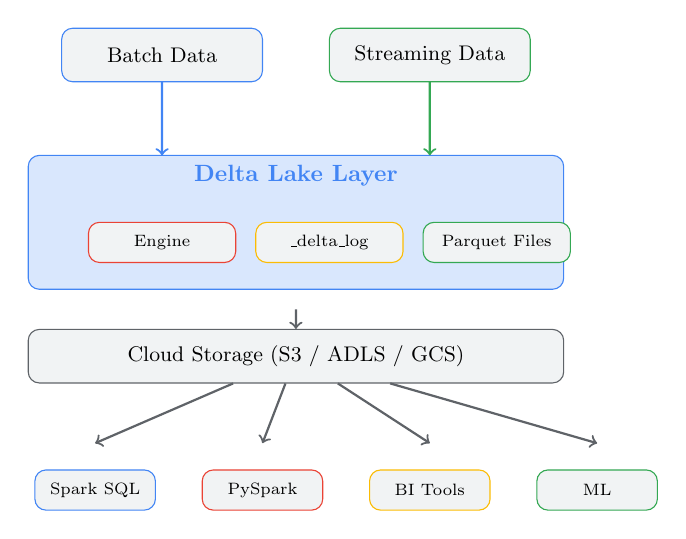
\begin{tikzpicture}[scale=0.85, transform shape]
            % Data Sources
            \node[draw=GoogleBlue, fill=GoogleLightGray, rounded corners, minimum width=3cm, minimum height=0.8cm] (batch) at (-4,3) {\small Batch Data};
            \node[draw=GoogleGreen, fill=GoogleLightGray, rounded corners, minimum width=3cm, minimum height=0.8cm] (stream) at (0,3) {\small Streaming Data};
            
            % Delta Lake Layer
            \node[draw=GoogleBlue, fill=GoogleBlue!20, rounded corners, minimum width=8cm, minimum height=2cm] (delta) at (-2,0.5) {};
            \node[font=\bfseries] at (-2,1.2) {\textcolor{GoogleBlue}{Delta Lake Layer}};
            \node[draw=GoogleRed, fill=GoogleLightGray, rounded corners, minimum width=2.2cm, minimum height=0.6cm] (engine) at (-4,0.2) {\scriptsize Engine};
            \node[draw=GoogleYellow, fill=GoogleLightGray, rounded corners, minimum width=2.2cm, minimum height=0.6cm] (log) at (-1.5,0.2) {\scriptsize \_delta\_log};
            \node[draw=GoogleGreen, fill=GoogleLightGray, rounded corners, minimum width=2.2cm, minimum height=0.6cm] (parquet) at (1,0.2) {\scriptsize Parquet Files};
            
            % Storage Layer
            \node[draw=GoogleGray, fill=GoogleLightGray, rounded corners, minimum width=8cm, minimum height=0.8cm] (storage) at (-2,-1.5) {\small Cloud Storage (S3 / ADLS / GCS)};
            
            % Consumers
            \node[draw=GoogleBlue, fill=GoogleLightGray, rounded corners, minimum width=1.8cm, minimum height=0.6cm] (sql) at (-5,-3.5) {\scriptsize Spark SQL};
            \node[draw=GoogleRed, fill=GoogleLightGray, rounded corners, minimum width=1.8cm, minimum height=0.6cm] (pyspark) at (-2.5,-3.5) {\scriptsize PySpark};
            \node[draw=GoogleYellow, fill=GoogleLightGray, rounded corners, minimum width=1.8cm, minimum height=0.6cm] (bi) at (0,-3.5) {\scriptsize BI Tools};
            \node[draw=GoogleGreen, fill=GoogleLightGray, rounded corners, minimum width=1.8cm, minimum height=0.6cm] (ml) at (2.5,-3.5) {\scriptsize ML};
            
            % Arrows
            \draw[->, thick, GoogleBlue] (batch) -- (-4,1.5);
            \draw[->, thick, GoogleGreen] (stream) -- (0,1.5);
            \draw[->, thick, GoogleGray] (-2,-0.8) -- (storage);
            \draw[->, thick, GoogleGray] (storage) -- (-5,-2.8);
            \draw[->, thick, GoogleGray] (storage) -- (-2.5,-2.8);
            \draw[->, thick, GoogleGray] (storage) -- (0,-2.8);
            \draw[->, thick, GoogleGray] (storage) -- (2.5,-2.8);
        \end{tikzpicture}
    \end{center}
\end{frame}

% ==========================================
% KEY FEATURES
% ==========================================
\begin{frame}{Delta Lake Key Features}
    \centering
    \small
    \begin{tabular}{>{\raggedright\arraybackslash}p{3.5cm}p{5.5cm}p{4cm}}
        \toprule
        \rowcolor{GoogleBlue!20}
        \textbf{Feature} & \textbf{Description} & \textbf{Benefit} \\
        \midrule
        \textcolor{GoogleBlue}{\faIcon{lock}} ACID Transactions & All operations are atomic and isolated & No partial writes \\
        \rowcolor{GoogleLightGray}
        \textcolor{GoogleRed}{\faIcon{shield-alt}} Schema Enforcement & Validates data against table schema & Prevents bad data \\
        \textcolor{GoogleGreen}{\faIcon{expand-arrows-alt}} Schema Evolution & Safely add new columns & Adapt to changes \\
        \rowcolor{GoogleLightGray}
        \textcolor{GoogleYellow}{\faIcon{history}} Time Travel & Query previous versions & Audit \& rollback \\
        \textcolor{GoogleBlue}{\faIcon{stream}} Unified Batch/Stream & Same table for both workloads & Simplified arch \\
        \rowcolor{GoogleLightGray}
        \textcolor{GoogleRed}{\faIcon{edit}} DML Operations & UPDATE, DELETE, MERGE & SQL-like operations \\
        \bottomrule
    \end{tabular}
\end{frame}

% ==========================================
% SECTION 2: ACID TRANSACTIONS
% ==========================================
\begin{frame}{ACID Transactions}
    \begin{tcolorbox}[googlebox, title={\textcolor{white}{What is ACID?}}]
        ACID stands for \textbf{Atomicity, Consistency, Isolation, and Durability} -- fundamental properties that ensure reliable transaction processing.
    \end{tcolorbox}
    
    \vspace{0.4cm}
    
    \begin{columns}[T]
        \begin{column}{0.5\textwidth}
            \textcolor{GoogleBlue}{\faIcon{atom}} \textbf{Atomicity}
            \begin{itemize}
                \item All or nothing
                \item No partial writes
            \end{itemize}
            
            \vspace{0.2cm}
            
            \textcolor{GoogleRed}{\faIcon{check-double}} \textbf{Consistency}
            \begin{itemize}
                \item Valid state to valid state
                \item Schema rules enforced
            \end{itemize}
        \end{column}
        \begin{column}{0.5\textwidth}
            \textcolor{GoogleGreen}{\faIcon{user-shield}} \textbf{Isolation}
            \begin{itemize}
                \item Transactions don't interfere
                \item Snapshot isolation for reads
            \end{itemize}
            
            \vspace{0.2cm}
            
            \textcolor{GoogleYellow}{\faIcon{save}} \textbf{Durability}
            \begin{itemize}
                \item Committed data persists
                \item Survives system failures
            \end{itemize}
        \end{column}
    \end{columns}
\end{frame}

% ==========================================
% ATOMICITY EXPLAINED
% ==========================================
\begin{frame}{Atomicity - All or Nothing}
    \begin{columns}[T]
        \begin{column}{0.48\textwidth}
            \textcolor{GoogleRed}{\faIcon{times-circle}} \textbf{Without Delta Lake}
            \begin{itemize}
                \item Job writes 1M records
                \item Crashes at 500K
                \item 500K records partially written
                \item Data corrupted, unusable
                \item Manual cleanup required
            \end{itemize}
        \end{column}
        \begin{column}{0.48\textwidth}
            \textcolor{GoogleGreen}{\faIcon{check-circle}} \textbf{With Delta Lake}
            \begin{itemize}
                \item Job writes 1M records
                \item Crashes at 500K
                \item Transaction not committed
                \item Partial files ignored
                \item Table remains valid!
            \end{itemize}
        \end{column}
    \end{columns}
    
    \vspace{0.5cm}
    
    \begin{tcolorbox}[colback=GoogleGreen!10, colframe=GoogleGreen, boxrule=1pt]
        \centering
        \textcolor{GoogleGreen}{\faIcon{lightbulb}} \textbf{Key Insight:} Delta Lake uses optimistic concurrency control with the transaction log to ensure atomic commits.
    \end{tcolorbox}
\end{frame}

% ==========================================
% ISOLATION - SNAPSHOT ISOLATION
% ==========================================
\begin{frame}{Isolation - Snapshot Consistency}
    \begin{tcolorbox}[googlebox, title={\textcolor{white}{How Snapshot Isolation Works}}]
        When you read a Delta table, you get a \textbf{consistent snapshot} at that point in time. Even if other processes are writing, your read sees the same data throughout.
    \end{tcolorbox}
    
    \vspace{0.3cm}
    
    \begin{center}
        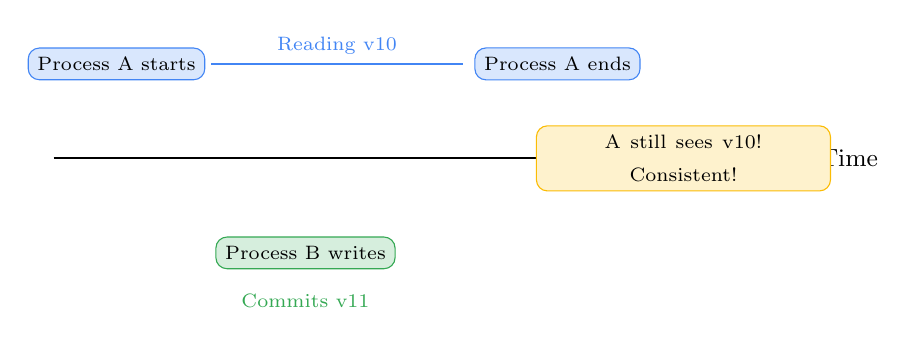
\begin{tikzpicture}[scale=0.8]
            % Timeline
            \draw[->, thick] (0,0) -- (12,0) node[right] {\small Time};
            
            % Process A
            \node[draw=GoogleBlue, fill=GoogleBlue!20, rounded corners] at (1,1.5) {\scriptsize Process A starts};
            \node[draw=GoogleBlue, fill=GoogleBlue!20, rounded corners] at (8,1.5) {\scriptsize Process A ends};
            \draw[thick, GoogleBlue] (2.5,1.5) -- (6.5,1.5);
            \node[above, GoogleBlue] at (4.5,1.5) {\scriptsize Reading v10};
            
            % Process B
            \node[draw=GoogleGreen, fill=GoogleGreen!20, rounded corners] at (4,-1.5) {\scriptsize Process B writes};
            \node[below, GoogleGreen] at (4,-2) {\scriptsize Commits v11};
            
            % Result
            \node[draw=GoogleYellow, fill=GoogleYellow!20, rounded corners, text width=3.5cm, align=center] at (10,0) {\scriptsize A still sees v10!\\\scriptsize Consistent!};
        \end{tikzpicture}
    \end{center}
\end{frame}

% ==========================================
% SECTION 3: SCHEMA ENFORCEMENT
% ==========================================
\begin{frame}{Schema Enforcement}
    \begin{tcolorbox}[googlebox, title={\textcolor{white}{Definition}}]
        Schema enforcement prevents \textbf{bad data from entering your tables} by validating incoming data matches the table schema exactly.
    \end{tcolorbox}
    
    \vspace{0.3cm}
    
    \textcolor{GoogleRed}{\faIcon{bug}} \textbf{The Schema Drift Problem}
    
    \begin{itemize}
        \item Week 1: Team A writes \texttt{\{"user\_id": 1, "name": "Alice"\}}
        \item Week 2: Team B writes \texttt{\{"userId": 2, "userName": "Bob"\}} \textcolor{GoogleRed}{← Different!}
        \item Week 3: Team C writes \texttt{\{"user\_id": "3", "name": "Charlie"\}} \textcolor{GoogleRed}{← Wrong type!}
        \item Week 4: \textcolor{GoogleRed}{\textbf{Dashboard breaks!}}
    \end{itemize}
    
    \vspace{0.3cm}
    
    \textcolor{GoogleGreen}{\faIcon{shield-alt}} \textbf{With Schema Enforcement:} Invalid writes are \textbf{rejected} immediately!
\end{frame}

% ==========================================
% SCHEMA VALIDATION RULES
% ==========================================
\begin{frame}{Schema Validation Rules}
    \centering
    \begin{tabular}{>{\raggedright\arraybackslash}p{3cm}p{5cm}p{3.5cm}}
        \toprule
        \rowcolor{GoogleBlue!20}
        \textbf{Check} & \textbf{What It Validates} & \textbf{On Failure} \\
        \midrule
        Column Names & All columns exist in table & Exception thrown \\
        \rowcolor{GoogleLightGray}
        Extra Columns & No unexpected columns & Exception thrown \\
        Data Types & Each column type matches & Exception thrown \\
        \rowcolor{GoogleLightGray}
        Nullability & NOT NULL columns have values & Exception thrown \\
        Column Order & N/A & Auto-handled \\
        \bottomrule
    \end{tabular}
    
    \vspace{0.5cm}
    
    \begin{tcolorbox}[colback=GoogleBlue!10, colframe=GoogleBlue, boxrule=1pt]
        \textcolor{GoogleBlue}{\faIcon{info-circle}} \textbf{Schema Evolution:} Use \texttt{mergeSchema=true} to safely add new columns when needed.
    \end{tcolorbox}
\end{frame}

% ==========================================
% SECTION 4: DELTA VS PARQUET
% ==========================================
\begin{frame}{Delta Lake vs Parquet}
    \centering
    \small
    \begin{tabular}{>{\raggedright\arraybackslash}p{3.5cm}cc}
        \toprule
        \rowcolor{GoogleBlue!20}
        \textbf{Feature} & \textbf{Parquet} & \textbf{Delta Lake} \\
        \midrule
        ACID Transactions & \textcolor{GoogleRed}{\faIcon{times}} & \textcolor{GoogleGreen}{\faIcon{check}} \\
        \rowcolor{GoogleLightGray}
        Schema Enforcement & \textcolor{GoogleRed}{\faIcon{times}} & \textcolor{GoogleGreen}{\faIcon{check}} \\
        Time Travel & \textcolor{GoogleRed}{\faIcon{times}} & \textcolor{GoogleGreen}{\faIcon{check}} \\
        \rowcolor{GoogleLightGray}
        UPDATE/DELETE & \textcolor{GoogleRed}{\faIcon{times}} & \textcolor{GoogleGreen}{\faIcon{check}} \\
        MERGE (Upsert) & \textcolor{GoogleRed}{\faIcon{times}} & \textcolor{GoogleGreen}{\faIcon{check}} \\
        \rowcolor{GoogleLightGray}
        Concurrent Writes & \textcolor{GoogleRed}{Can corrupt} & \textcolor{GoogleGreen}{Safe} \\
        Streaming Support & \textcolor{GoogleYellow}{Limited} & \textcolor{GoogleGreen}{\faIcon{check}} \\
        \rowcolor{GoogleLightGray}
        Small File Problem & \textcolor{GoogleRed}{Common} & \textcolor{GoogleGreen}{Auto-compact} \\
        Audit History & \textcolor{GoogleRed}{\faIcon{times}} & \textcolor{GoogleGreen}{\faIcon{check}} \\
        \bottomrule
    \end{tabular}
\end{frame}

% ==========================================
% UPDATE COMPARISON
% ==========================================
\begin{frame}[fragile]{Data Modification: Parquet vs Delta}
    \begin{columns}[T]
        \begin{column}{0.48\textwidth}
            \textcolor{GoogleRed}{\faIcon{times-circle}} \textbf{Parquet (Complex)}
            \begin{lstlisting}[language=Python, basicstyle=\ttfamily\tiny]
# Must rewrite entire table!
df = spark.read.parquet("/path")
keep = df.filter("id != 1")
update = df.filter("id = 1")
updated = update.withColumn(
    "price", lit(899.99))
final = keep.union(updated)
final.write.mode("overwrite")
    .parquet("/path")
# Not atomic, slow, risky!
            \end{lstlisting}
        \end{column}
        \begin{column}{0.48\textwidth}
            \textcolor{GoogleGreen}{\faIcon{check-circle}} \textbf{Delta Lake (Simple)}
            \begin{lstlisting}[language=Python, basicstyle=\ttfamily\tiny]
from delta.tables import DeltaTable

delta_table = DeltaTable.forPath(
    spark, "/delta/products")

# Simple, atomic UPDATE
delta_table.update(
    condition="id = 1",
    set={"price": "899.99"}
)
# Atomic, fast, safe!
            \end{lstlisting}
        \end{column}
    \end{columns}
\end{frame}

% ==========================================
% TIME TRAVEL
% ==========================================
\begin{frame}[fragile]{Time Travel Capability}
    \begin{tcolorbox}[googlebox, title={\textcolor{white}{Query Historical Data}}]
        Delta Lake maintains a complete history of all changes, enabling you to query any previous version.
    \end{tcolorbox}
    
    \vspace{0.3cm}
    
    \begin{lstlisting}[language=Python, basicstyle=\ttfamily\scriptsize]
# Query data as it existed yesterday
df_yesterday = spark.read.format("delta") \
    .option("timestampAsOf", "2024-01-14") \
    .load("/delta/data")

# Query specific version
df_v5 = spark.read.format("delta") \
    .option("versionAsOf", 5) \
    .load("/delta/data")

# See all versions
spark.sql("DESCRIBE HISTORY delta.`/delta/data`")
    \end{lstlisting}
    
    \vspace{0.2cm}
    
    \textcolor{GoogleYellow}{\faIcon{lightbulb}} Use cases: Audit trails, rollback mistakes, reproduce ML experiments
\end{frame}

% ==========================================
% TASK 1: CSV TO DELTA
% ==========================================
\begin{frame}[fragile]{Task 1: Convert CSV to Delta}
    \begin{lstlisting}[language=Python, basicstyle=\ttfamily\scriptsize]
# Define schema for CSV reading
csv_schema = StructType([
    StructField("employee_id", IntegerType(), nullable=False),
    StructField("name", StringType(), nullable=False),
    StructField("department", StringType(), nullable=True),
    StructField("salary", DoubleType(), nullable=True),
    StructField("hire_date", DateType(), nullable=True)
])

# Read CSV with explicit schema
csv_df = spark.read.option("header", "true") \
    .schema(csv_schema).csv("/data/csv/employees")

# Convert to Delta format
csv_df.write.format("delta") \
    .mode("overwrite").save("/delta/employees")

print("Successfully converted CSV to Delta!")
    \end{lstlisting}
\end{frame}

% ==========================================
% TASK 2: CREATE DELTA TABLES
% ==========================================
\begin{frame}[fragile]{Task 2: Create Delta Tables}
    \begin{columns}[T]
        \begin{column}{0.48\textwidth}
            \textcolor{GoogleBlue}{\faIcon{python}} \textbf{PySpark Method}
            \begin{lstlisting}[language=Python, basicstyle=\ttfamily\tiny]
products_df = spark.createDataFrame([
    (101, "Laptop", 1299.99),
    (102, "Mouse", 29.99)
], ["id", "name", "price"])

products_df.write \
    .format("delta") \
    .mode("overwrite") \
    .save("/delta/products")
            \end{lstlisting}
        \end{column}
        \begin{column}{0.48\textwidth}
            \textcolor{GoogleGreen}{\faIcon{database}} \textbf{SQL Method}
            \begin{lstlisting}[language=SQL, basicstyle=\ttfamily\tiny]
CREATE TABLE default.orders (
    order_id INT NOT NULL,
    customer_id INT NOT NULL,
    amount DOUBLE,
    order_date DATE
)
USING DELTA
LOCATION '/delta/orders';

INSERT INTO default.orders 
VALUES (1001, 501, 1299.99, 
        '2024-01-10');
            \end{lstlisting}
        \end{column}
    \end{columns}
    
    \vspace{0.3cm}
    
    \begin{tcolorbox}[colback=GoogleYellow!10, colframe=GoogleYellow, boxrule=1pt]
        \textcolor{GoogleYellow}{\faIcon{lightbulb}} \textbf{Pro Tip:} Use \texttt{partitionBy()} for large tables to improve query performance!
    \end{tcolorbox}
\end{frame}

% ==========================================
% TASK 3: SCHEMA ENFORCEMENT TEST
% ==========================================
\begin{frame}[fragile]{Task 3: Schema Enforcement in Action}
    \textcolor{GoogleRed}{\faIcon{exclamation-triangle}} \textbf{Test: Wrong Data Type}
    \begin{lstlisting}[language=Python, basicstyle=\ttfamily\scriptsize]
# Table schema: price is DOUBLE
bad_data = spark.createDataFrame([
    (106, "Keyboard", "fifty nine")  # String instead of Double!
], ["product_id", "product_name", "price"])

try:
    bad_data.write.format("delta").mode("append").save("/delta/products")
except Exception as e:
    print("Schema enforcement blocked write!")
    # Error: Failed to merge incompatible types DoubleType and StringType
    \end{lstlisting}
    
    \vspace{0.3cm}
    
    \textcolor{GoogleGreen}{\faIcon{check-circle}} \textbf{Result:} Bad data is \textbf{rejected} -- table integrity preserved!
    
    \vspace{0.2cm}
    
    \textcolor{GoogleBlue}{\faIcon{info-circle}} Enable schema evolution with: \texttt{.option("mergeSchema", "true")}
\end{frame}

% ==========================================
% TASK 4: MERGE OPERATION
% ==========================================
\begin{frame}[fragile]{Task 4: Handle Duplicates with MERGE}
    \begin{lstlisting}[language=Python, basicstyle=\ttfamily\scriptsize]
from delta.tables import DeltaTable

delta_table = DeltaTable.forPath(spark, "/delta/customers")

# Incoming data (may contain duplicates)
incoming_df = spark.createDataFrame([
    (1, "Alice", "alice_new@email.com"),  # Existing
    (4, "David", "david@email.com")        # New
], ["customer_id", "name", "email"])

# MERGE: Update existing, insert new
delta_table.alias("target").merge(
    incoming_df.alias("source"),
    "target.customer_id = source.customer_id"
).whenMatchedUpdateAll() \
 .whenNotMatchedInsertAll() \
 .execute()
    \end{lstlisting}
    
    \begin{tcolorbox}[colback=GoogleGreen!10, colframe=GoogleGreen, boxrule=1pt]
        \textcolor{GoogleGreen}{\faIcon{check}} Existing records updated, new records inserted -- atomically!
    \end{tcolorbox}
\end{frame}

% ==========================================
% MERGE STRATEGIES
% ==========================================
\begin{frame}{MERGE Strategies Overview}
    \centering
    \begin{tabular}{>{\raggedright\arraybackslash}p{3.5cm}p{5cm}p{3.5cm}}
        \toprule
        \rowcolor{GoogleBlue!20}
        \textbf{Strategy} & \textbf{Behavior} & \textbf{Use Case} \\
        \midrule
        \textcolor{GoogleBlue}{Insert Only New} & Skip duplicates, insert new & Deduplication \\
        \rowcolor{GoogleLightGray}
        \textcolor{GoogleGreen}{Upsert} & Update existing + insert new & Sync data sources \\
        \textcolor{GoogleYellow}{Conditional Update} & Update specific columns only & Partial updates \\
        \rowcolor{GoogleLightGray}
        \textcolor{GoogleRed}{Delete \& Replace} & Replace entire groups & Batch reprocessing \\
        \bottomrule
    \end{tabular}
    
    \vspace{0.5cm}
    
    \begin{columns}[T]
        \begin{column}{0.5\textwidth}
            \textcolor{GoogleBlue}{\faIcon{check-circle}} \textbf{Benefits}
            \begin{itemize}
                \item Single atomic operation
                \item No data duplication
                \item Handles complex scenarios
            \end{itemize}
        \end{column}
        \begin{column}{0.5\textwidth}
            \textcolor{GoogleGreen}{\faIcon{code}} \textbf{SQL Alternative}
            \begin{itemize}
                \item \texttt{MERGE INTO ... USING ...}
                \item \texttt{WHEN MATCHED THEN UPDATE}
                \item \texttt{WHEN NOT MATCHED THEN INSERT}
            \end{itemize}
        \end{column}
    \end{columns}
\end{frame}

% ==========================================
% QUICK REFERENCE
% ==========================================
\begin{frame}[fragile]{Quick Reference: Essential Commands}
    \begin{columns}[T]
        \begin{column}{0.48\textwidth}
            \textcolor{GoogleBlue}{\faIcon{file-import}} \textbf{Read Data}
            \begin{lstlisting}[language=Python, basicstyle=\ttfamily\tiny]
# Basic read
df = spark.read.format("delta")
    .load("/path")

# Time travel by version
df = spark.read.format("delta")
    .option("versionAsOf", 5)
    .load("/path")

# Time travel by timestamp
df = spark.read.format("delta")
    .option("timestampAsOf", 
            "2024-01-10")
    .load("/path")
            \end{lstlisting}
        \end{column}
        \begin{column}{0.48\textwidth}
            \textcolor{GoogleGreen}{\faIcon{file-export}} \textbf{Write Data}
            \begin{lstlisting}[language=Python, basicstyle=\ttfamily\tiny]
# Overwrite
df.write.format("delta")
    .mode("overwrite")
    .save("/path")

# Append
df.write.format("delta")
    .mode("append")
    .save("/path")

# With schema evolution
df.write.format("delta")
    .option("mergeSchema", "true")
    .mode("append").save("/path")
            \end{lstlisting}
        \end{column}
    \end{columns}
\end{frame}

% ==========================================
% SQL QUICK REFERENCE
% ==========================================
\begin{frame}[fragile]{Quick Reference: SQL Commands}
    \begin{lstlisting}[language=SQL, basicstyle=\ttfamily\scriptsize]
-- Create table
CREATE TABLE my_table (id INT, name STRING) USING DELTA LOCATION '/path';

-- Insert data
INSERT INTO my_table VALUES (1, 'Alice');

-- Update records
UPDATE delta.`/path` SET name = 'Bob' WHERE id = 1;

-- Delete records  
DELETE FROM delta.`/path` WHERE id = 1;

-- MERGE (upsert)
MERGE INTO target USING source ON target.id = source.id
WHEN MATCHED THEN UPDATE SET *
WHEN NOT MATCHED THEN INSERT *;

-- Time travel
SELECT * FROM delta.`/path` VERSION AS OF 5;

-- View history
DESCRIBE HISTORY delta.`/path`;
    \end{lstlisting}
\end{frame}

% ==========================================
% SUMMARY SLIDE
% ==========================================
\begin{frame}{Summary: Delta Lake Benefits}
    \begin{center}
        \begin{tikzpicture}[scale=0.9]
            % Central node
            \node[draw=GoogleBlue, fill=GoogleBlue!20, rounded corners, minimum width=3.5cm, minimum height=1.2cm, font=\large\bfseries] (center) at (0,0) {Delta Lake};
            
            % Surrounding benefits
            \node[draw=GoogleBlue, fill=GoogleBlue!10, rounded corners, text width=2.8cm, align=center] (acid) at (-4,2) {\faIcon{lock}\\ACID\\Transactions};
            \node[draw=GoogleRed, fill=GoogleRed!10, rounded corners, text width=2.8cm, align=center] (schema) at (0,3) {\faIcon{shield-alt}\\Schema\\Enforcement};
            \node[draw=GoogleGreen, fill=GoogleGreen!10, rounded corners, text width=2.8cm, align=center] (time) at (4,2) {\faIcon{history}\\Time\\Travel};
            \node[draw=GoogleYellow, fill=GoogleYellow!10, rounded corners, text width=2.8cm, align=center] (unified) at (-4,-2) {\faIcon{stream}\\Unified\\Batch/Stream};
            \node[draw=GoogleGreen, fill=GoogleGreen!10, rounded corners, text width=2.8cm, align=center] (dml) at (4,-2) {\faIcon{edit}\\Full DML\\Support};
            
            % Connections
            \draw[->, thick, GoogleBlue] (center) -- (acid);
            \draw[->, thick, GoogleRed] (center) -- (schema);
            \draw[->, thick, GoogleGreen] (center) -- (time);
            \draw[->, thick, GoogleYellow] (center) -- (unified);
            \draw[->, thick, GoogleGreen] (center) -- (dml);
        \end{tikzpicture}
    \end{center}
    
    \vspace{0.3cm}
    
    \begin{tcolorbox}[colback=GoogleBlue!10, colframe=GoogleBlue, boxrule=1pt]
        \centering
        \textbf{Key Insight:} Delta Lake achieves database-like reliability by adding a \textbf{transaction log} alongside Parquet files -- simple yet powerful!
    \end{tcolorbox}
\end{frame}

% ==========================================
% THANK YOU SLIDE
% ==========================================
{
\setbeamertemplate{footline}{}
\begin{frame}[plain]
    \begin{tikzpicture}[remember picture,overlay]
        \fill[GoogleBlue] (current page.north west) rectangle (current page.south east);
        \fill[GoogleRed,opacity=0.3] (10,-4) circle (4cm);
        \fill[GoogleYellow,opacity=0.3] (-3,2) circle (3cm);
        \fill[GoogleGreen,opacity=0.3] (13,3) circle (2.5cm);
    \end{tikzpicture}
    
    \begin{center}
        \vspace{2cm}
        {\Huge\bfseries\textcolor{GoogleWhite}{Thank You!}}
        
        \vspace{1cm}
        
        {\Large\textcolor{GoogleYellow}{Questions?}}
        
        \vspace{1.5cm}
        
        \textcolor{GoogleWhite}{\faIcon{linkedin} \href{https://www.linkedin.com/in/yashkavaiya}{linkedin.com/in/yashkavaiya}}
        
        \vspace{0.3cm}
        
        \textcolor{GoogleWhite}{\faIcon{globe} \href{https://easy-ai-labs.lovable.app/}{easy-ai-labs.lovable.app}}
        
        \vspace{0.3cm}
        
        \textcolor{GoogleWhite}{\faIcon{graduation-cap} \href{https://www.linkedin.com/company/genai-guru}{Gen AI Guru}}
    \end{center}
\end{frame}
}

\end{document}
